\documentclass{beamer}

\usetheme{default}

\usefonttheme{structurebold}
\usepackage{helvet}
\usecolortheme{seagull}         % white on black

\usepackage[utf8]{inputenc}
\PassOptionsToPackage{hyphens}{url}\usepackage{hyperref,xspace,multicol}
\usepackage[absolute,overlay]{textpos}
\usepackage{tikz}
\usetikzlibrary{arrows,shapes,trees,shadows,positioning}
%% \usepackage{tree}
\usepackage{fancyvrb}           % for \Verb
\usepackage{ulem}               % for \sout

% Remember the position of every picture.
\tikzstyle{every picture}+=[remember picture]

\tikzset{onslide/.code args={<#1>#2}{%
  \only<#1>{\pgfkeysalso{#2}} % \pgfkeysalso doesn't change the path
}}

% Colors.
\definecolor{guixred1}{RGB}{226,0,38}  % red P
\definecolor{guixorange1}{RGB}{243,154,38}  % guixorange P
\definecolor{guixyellow}{RGB}{254,205,27}  % guixyellow P
\definecolor{guixred2}{RGB}{230,68,57}  % red S
\definecolor{guixorange2}{RGB}{236,117,40}  % guixorange S
\definecolor{guixtaupe}{RGB}{134,113,127} % guixtaupe S
\definecolor{guixgrey}{RGB}{91,94,111} % guixgrey S
\definecolor{guixblue1}{RGB}{38,109,131} % guixblue S
\definecolor{guixblue2}{RGB}{10,50,80} % guixblue S
\definecolor{guixgreen1}{RGB}{133,146,66} % guixgreen S
\definecolor{guixgreen2}{RGB}{157,193,7} % guixgreen S

\setbeamerfont{title}{size=\huge}
\setbeamerfont{frametitle}{size=\huge}

% Black-on-white color theme.
\setbeamercolor{structure}{fg=guixblue2}
\setbeamercolor{title}{fg=guixblue2}
\setbeamercolor{frametitle}{fg=guixblue2}
\setbeamercolor{date}{fg=darkgray}
\setbeamercolor{author}{fg=darkgray}
\setbeamercolor{alerted text}{fg=guixgreen2,bg=black}

\title{Functional Package Management with GNU Guix}
%%\subtitle{How GNU Guix Seeks to Empower Users}

\author{Ricardo Wurmus\\\texttt{rekado@elephly.net}}
\date{\small{OpenTechSummit\\14 May 2015}}

\setbeamertemplate{navigation symbols}{} % remove the navigation bar

\AtBeginSection[]{
  \begin{frame}
    \frametitle{}
    \tableofcontents[currentsection, hideothersections]
  \end{frame} 
}


\AtBeginSubsection[]{
  \begin{frame}
  \frametitle{}
  \tableofcontents[currentsection, currentsubsection]
  \end{frame}
}

\begin{document}

\maketitle

\begin{frame}{Good idea}
  \Large{
  \begin{itemize}
  \item easy to install, upgrade, remove software
  \item dependency resolution
  \item centrally maintained repositories
  \end{itemize}
  }
\end{frame}

\begin{frame}{Common problems}
  \Large{
  \begin{itemize}
  \item outdated packages
  \item version conflicts
  \item changes affect all users
  \item potentially dangerous
  \item trust
  \end{itemize}
  }
\end{frame}

\begin{frame}{Partial solutions}
  \setbeamercovered{transparent=35}

  \Large{
  \begin{itemize}[<+>]
  \item \alert{third-party repositories}\\
        EPEL, PPAs, ...
  \item \alert{manual compilation}\\
        install to custom prefix, static linking
  \item \alert{language-specific package systems}\\
        gem, cabal, pip, cpan, npm ...
  \item \alert{build your own system package}\\
        RPM, deb, PKGBUILD, ...
  \item \alert{meta package managers}\\
        e.g. fpm generating RPM, deb, gem
  \item \alert{giving up}\\
        virtual machines, ``app images'', snapshots
  \end{itemize}
  }
\end{frame}

\begin{frame}[plain]
  \includegraphics[width=\textwidth]{images/guix-logo}
\end{frame}

\begin{frame}[plain]
  \begin{center}
    \includegraphics[height=0.6\textheight]{images/function}
  \end{center}
\end{frame}

\begin{frame}[plain]
  \begin{center}
    \includegraphics[height=0.8\textheight]{images/functional-package}
  \end{center}
\end{frame}

\begin{frame}{Functional package management}
  \Large{
  \begin{itemize}
  \item no \alert{global} values:\\
        /bin, /usr/include, /usr/lib, ...
  \item \alert{purity}:\\
        only declared inputs are visible at build time
  \item \alert{reproducible} results:\\
        build outputs can be cached and substituted;\\
        automatic deduplication!
  \item \alert{immutable results} without \alert{side effects}:\\
        nothing outside of the cache and internal state is modified
  \end{itemize}
  }
\end{frame}

\begin{frame}[fragile]{}
  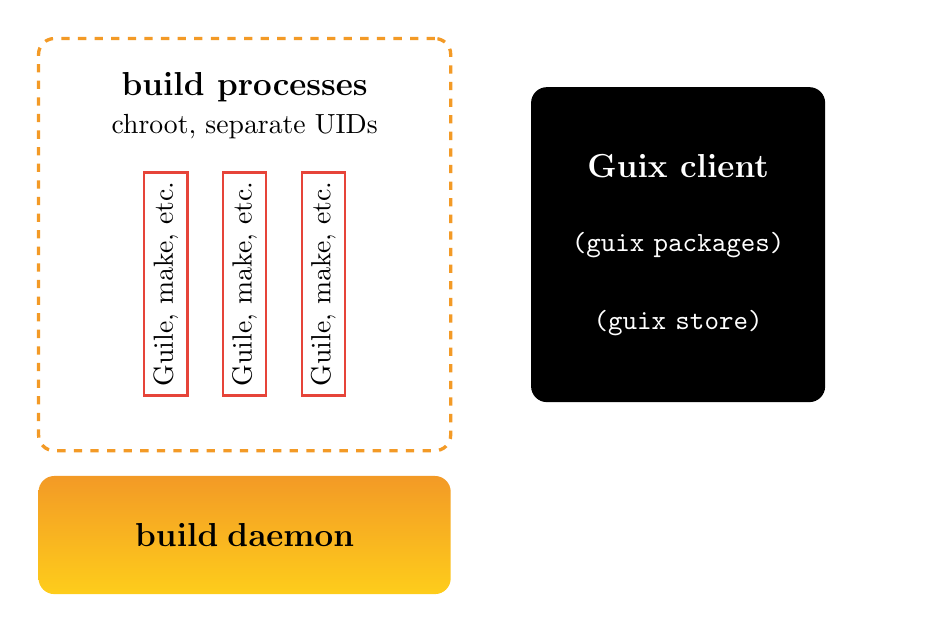
\begin{tikzpicture}[tools/.style = {
                        text width=35mm, minimum height=4cm,
                        text centered,
                        rounded corners=2mm,
                        fill=black, text=white
                      },
                      tool/.style = {
                        fill=black, text=white, text width=3cm,
                        text centered
                      },
                      daemon/.style = {
                        rectangle, text width=50mm, text centered,
                        rounded corners=2mm, minimum height=15mm,
                        top color=guixorange1,
                        bottom color=guixyellow,
                        text=black
                      },
                      builders/.style = {
                        draw=guixorange1, very thick, dashed,
                        fill=white, text=black, text width=5cm,
                        rounded corners=2mm,
                      },
                      builder/.style = {
                        draw=guixred2, thick, rectangle,
                        fill=white, text=black,
                        rotate=90
                      }]
    \matrix[row sep=3mm, column sep=1cm] {
      \node(builders)[builders, text height=5cm]{}
          node at (0, 2) {\large{\textbf{build processes}}}
          node at (0, 1.5) {chroot, separate UIDs}
          node[builder] at (-1,-0.5) {\alert{Guile}, make, etc.}
          node[builder] at ( 0,-0.5) {\alert{Guile}, make, etc.}
          node[builder] at ( 1,-0.5) {\alert{Guile}, make, etc.}; &
      \node[tools]{}
          node[text=white] at (0, 1) {\large{\textbf{Guix client}}}
          node[tool] at (0, 0) {\texttt{(guix packages)}}
          node(client)[tool] at (0, -1) {\texttt{(guix store)}};
      \\

      \node(daemon)[daemon]{\large{\textbf{build daemon}}}; &
      &
      \\
    };
  \end{tikzpicture}

  \begin{tikzpicture}[overlay]
    \path[very thick, draw=guixblue2]
      (client.south) edge [out=-90, in=0, ->] node[below, sloped]{RPCs} (daemon.east);
    \path[->, very thick, draw=guixblue2]
      (daemon) edge (builders);
  \end{tikzpicture}
\end{frame}

\begin{frame}[plain]
  \begin{center}
    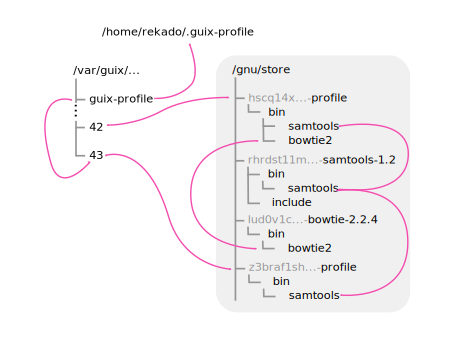
\includegraphics[height=\textheight]{images/profile-1}
  \end{center}
\end{frame}
\begin{frame}[plain]
  \begin{center}
    \includegraphics[height=\textheight]{images/profile-2}
  \end{center}
\end{frame}

\begin{frame}[fragile]
  \begin{semiverbatim}
(define hello
  (\alert{package}
   (name "hello")
   (version "2.8")
   (source (\alert{origin}
            (method url-fetch)
            (uri (string-append
                  "mirror://gnu/\textrm{...}/hello-" version
                  ".tar.gz"))
            (sha256 (base32 "0wqd\textrm{...}dz6"))))
   (\alert{build-system} gnu-build-system)
   (synopsis "Hello, GNU world: An example GNU package")
   (description "Produce a friendly greeting.")
   (home-page "http://www.gnu.org/software/hello/")
   (license gpl3+)))
  \end{semiverbatim}
\end{frame}

\begin{frame}[plain]

  \vspace{0.7cm}
  \Large{
    \begin{itemize}
    \item version 0.8.2 is \textbf{out now}
    \item quickly growing collection of package recipes (1800+)
    \item \textbf{install the distribution}
    \item \textbf{use it}, report bugs, add packages
    \item share your \textbf{ideas}!
    \end{itemize}
  }

  \begin{textblock}{5}(7,8)
    \tikz
    \node[overlay, rounded corners=4, text centered,
          minimum size=10mm, fill=guixorange1, text width=5cm,
          inner sep=3mm, rotate=-7, opacity=.75, text opacity=1,
          drop shadow={opacity=0.5}] at (3, 3) {
            \textbf{your help needed!}
          };
  \end{textblock}
\end{frame}

\begin{frame}{}
\hfill{
  \includegraphics[width=0.5\textwidth]{images/gnuhead}
  \includegraphics[width=0.5\textwidth]{images/guixsd-logo}}
\vfill{
  \hfill{\includegraphics[width=0.3\textwidth]{images/guix-logo}}\\[0.2cm]
  \texttt{rekado@elephly.net} \hfill{\alert{\url{http://gnu.org/software/guix/}}}
}

\end{frame}

\begin{frame}{}

  \begin{textblock}{12}(2, 8)
    \tiny{
      Copyright \copyright{} 2015 Ricardo Wurmus \texttt{rekado@elephly.net}.\\
      Copyright \copyright{} 2010, 2012, 2013, 2014 Ludovic Courtès \texttt{ludo@gnu.org}.
      \\[3.0mm]
      A GNU head, GFDL, \url{http://gnu.org/graphics/agnuhead.html}\\
      GNU Guix logo, GFDL, \url{http://gnu.org/s/guix/graphics}

      Copyright of other images included in this document is held by
      their respective owners.
      \\[3.0mm]
      This work is licensed under the \alert{Creative Commons
        Attribution-Share Alike 3.0} License.  To view a copy of this
      license, visit
      \url{http://creativecommons.org/licenses/by-sa/3.0/} or send a
      letter to Creative Commons, 171 Second Street, Suite 300, San
      Francisco, California, 94105, USA.
      \\[2.0mm]
      At your option, you may instead copy, distribute and/or modify
      this document under the terms of the \alert{GNU Free Documentation
        License, Version 1.3 or any later version} published by the Free
      Software Foundation; with no Invariant Sections, no Front-Cover
      Texts, and no Back-Cover Texts.  A copy of the license is
      available at \url{http://www.gnu.org/licenses/gfdl.html}.
      \\[2.0mm]
      % Give a link to the 'Transparent Copy', as per Section 3 of the GFDL.
      The source of this document is available from
      \url{http://git.sv.gnu.org/cgit/guix/maintenance.git}.
    }
  \end{textblock}
\end{frame}

\end{document}

% Local Variables:
% coding: utf-8
% comment-start: "%"
% comment-end: ""
% ispell-local-dictionary: "american"
% compile-command: "pdflatex talk.tex"
% End:
